\documentclass[12pt]{article}

% This first part of the file is called the PREAMBLE. It includes
% customizations and command definitions. The preamble is everything
% between \documentclass and \begin{document}.

\usepackage[margin=1in]{geometry}  % set the margins to 1in on all sides
\usepackage{graphicx}              % to include figures
\usepackage{amsmath}               % great math stuff
\usepackage{amsfonts}              % for blackboard bold, etc
\usepackage{amsthm}                % better theorem environments
\usepackage{amssymb} 
\usepackage{mathptmx}
\usepackage{enumerate}
\usepackage{listings}
\usepackage{xcolor}
\usepackage{forest}
\usepackage{tabularx}  

% various theorems, numbered by section

\newtheorem{thm}{Theorem}[section]
\newtheorem{lem}[thm]{Lemma}
\newtheorem{prop}[thm]{Proposition}
\newtheorem{cor}[thm]{Corollary}
\newtheorem{conj}[thm]{Conjecture}
\newtheorem{mydef}[thm]{Definition}
\lstset{
	basicstyle          =   \sffamily,          
	keywordstyle        =   \bfseries,          
	commentstyle        =   \rmfamily\itshape,  
	stringstyle         =   \ttfamily,  
	flexiblecolumns,                
	numbers             =   left,   
	showspaces          =   false,  
	numberstyle         =   \fontsize{5}{skip},    
	showstringspaces    =   false,
	captionpos          =   t,      
	frame               =   lrtb,   
}

\lstdefinestyle{cpp}{
	language        =   cpp, 
	basicstyle      =   \fontsize{5}{skip},
	numberstyle     =   \fontsize{5}{skip},
	keywordstyle    =   \color{blue},
	keywordstyle    =   [2] \color{teal},
	stringstyle     =   \color{magenta},
	commentstyle    =   \color{red}\ttfamily,
	breaklines      =   true,   
	columns         =   fixed,  
	basewidth       =   0.5em,
}
\begin{document}


\title{ CSE 102 Spring 2021\\
	Quiz Reflection 2}

\author{Jaden Liu \\ 
University of California at Santa Cruz\\
Santa Cruz, CA 95064 USA }

\maketitle


\section{Quiz 2} 
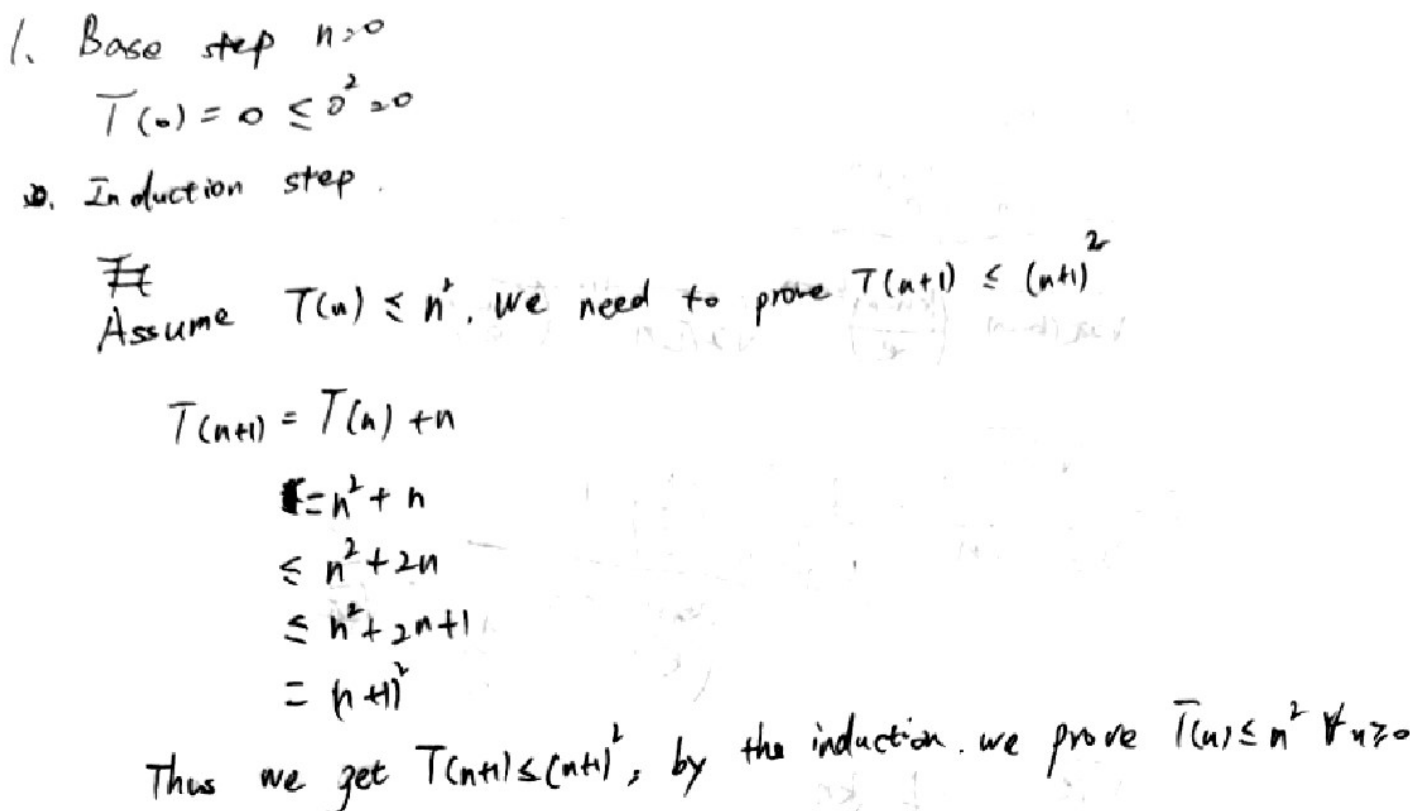
\includegraphics[scale=0.35]{1.png}
\begin{proof}[Solution]
	I changed the relation between $T(n)+n$ and $n^2 + n$ from $<$ to $=$ in the last minute. I don't know what I was thinking about at that time. Also, $T(n+1)$ should be equal to $T(n)+n+1$.
	Thus, the whole solution should be like this:\\
	Base case: n=0\\
	T(0) = 0  $\le0^2$\\
	Induction step:
	\begin{align*}
		T(n+1)&=T(n)+n+1\\
		&\le n^2+n+1\\
		&\le n^2+2n+1\\
		&=(n+1)^2
	\end{align*}
Thus, we get $T(n+1)\le(n+1)^2$. By the induction, we prove that $T(n)\le n^2$.
\end{proof}
\bigskip




\begin{thebibliography}{so}
\bibitem{so} 
\end{thebibliography}


\end{document}
